\documentclass{article}
\usepackage[utf8]{inputenc}
\usepackage{tikz} %package for plots, graphics and functions

\title{Plotting Functions}
\author{Arman Daneshdoost}
\date{March 2024}

\begin{document}
	\maketitle
	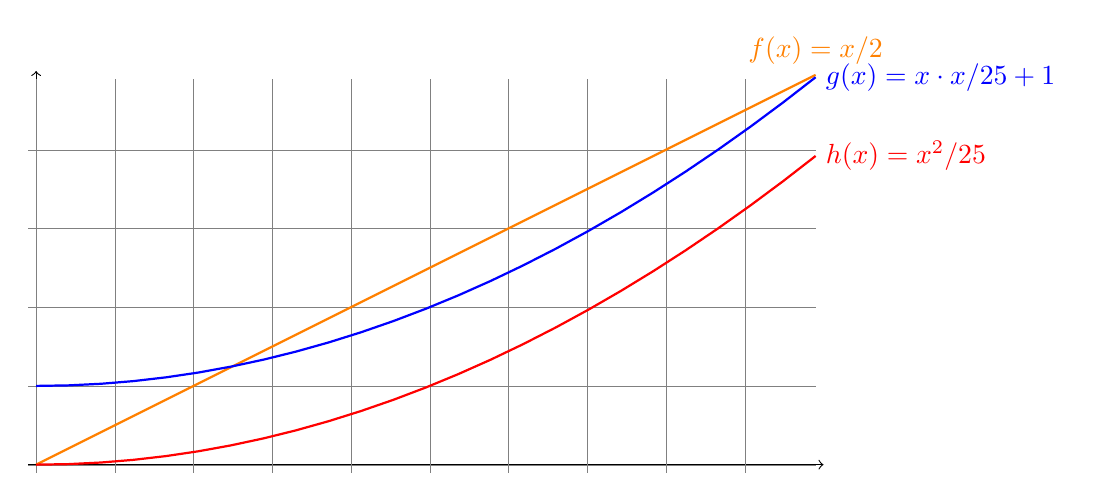
\begin{tikzpicture}[domain = 0 : 9.9]
		\draw[ -> ] (-0.1, 0) -- (10, 0);
		\draw [ ->] (0, -0.1) -- (0, 5);
		\draw [gray, ultra thin] (-0.1, -0.1) grid (9.9, 4.9); %draw grids
		
		\draw [orange, thick] plot (\x, \x/2) node[above] {$f(x) = x/2$};
		\draw [blue, thick] plot (\x, \x * \x / 25 + 1) node [right]{$g(x) = x \cdot x/25 + 1$};
		\draw [red, thick] plot (\x, {pow(\x, 2)/25}) node [right] {$h(x) = x ^ 2/25$};
	\end{tikzpicture}

	\begin{tikzpicture}
		\draw [ ->] (-1.6, 0) -- (1.6, 0);
		\draw [ ->] (0, -0.1) -- (0, 4.9);
		\draw [brown, thick, domain = -1.5:1.5] plot (\x, {exp(\x)}) node[right] {$\exp(x)$};
	\end{tikzpicture}
\end{document}